
\chapter{二八原则} % Introduction chapter suppressed from the table of contents

团队成员协作，利用项目数据，分析根本原因，制定纠正措施，并立马尝试，判断是否有效，是改善的``基本功''。10-12章会探索里面的注意事项，13章会看两家公司的实施情况和常见问题。\\
如果已经获得高层支持，高层赞同目前返工工作量太多并愿意投入资源进行过程改进，我们首先应该针对哪些方面进行改进呢？\\
软件开发的特点是，超过95\%的成本都是人力成本。因此，我一般会从二八(20/80)原则开始（附件里有二八原则简介），识别应针对什么做改进，才能最容易取得效果。软件开发里什么工作的占比最高？\\

\framebox{%
\begin{minipage}[t]{0.97\columnwidth}\raggedright
\textbf{请把过去一年的软件开发项目，按照不同工种占项目总工作量的比例，从多到少排个序。}

\begin{enumerate}
\tightlist
\item
  编码与代码设计
\item
  交付后的所有工作，包括维护、更新与缺陷修正
\item
  交付前的评审，静态扫描，测试与缺陷修正
\item
  项目管理与监控
\end{enumerate}
\strut
\end{minipage}}

可以参考软件开发度量专家卡铂斯•琼斯 (Capers Jones)
先生在2012年的研究（详见附件中的``开发项目工作量(成本)分布''），看看你的选择与典型分布有多大差距。\\
软件开发项目最大的工作量通常是花在找出与修正缺陷上（开发里的``测试与评审''），Capers
Jones
发现，对于一个超过10,000个功能点、计划使用25年的大型系统来说，有接近一半的工作量是与找出并修正缺陷相关。\\
很多项目中的缺陷大部分还是到后期才发现，这导致了大量返工。如果能提前发现并解决这些缺陷，就可以大大降低研发成本(不仅仅是提升产品质量)。\\
对于一个软件项目来说，发现缺陷最多的是在系统测试阶段，其次是在验收测试阶段（很多公司都是如此）：\\
\url{文件:微信截图_20231023085822.png}

但很多开发人员误以为编码是项目的主要工作，却忽视了大量因质量问题引起的返工。\\
前面在``获取高层支持''那章里缺陷越后面发现，返工量越高，如果是在前面评审或单元测试发现的缺陷返工量不会超过一小时，但到了系统测试或验收，返工量平均不会低于２０人时。所以在软件开发，大量缺陷在后面测试或客户使用时才发现不单影响产品质量，也会导致大量返工。\\
只有当管理层意识到尽早发现并排除缺陷的重要性并引起重视，公司才有机会改进。

\framebox{%
\begin{minipage}[t]{0.97\columnwidth}\raggedright
有些偏业务的领导可能会质疑，客户不一定关注缺陷密度，只要达到可接受的水平就可以了。\\
我解释：``在软件开发中，减少后期测试才发现的缺陷，不仅仅能提升产品质量，更重要的是能降低研发的总工作量，所以最终能帮助公司省钱，减少开发人员加班。''（详见附件``公司高层不一定关注质量''）
\strut
\end{minipage}}

\hypertarget{ux600eux6837ux5f00ux59cb}{%
\subsection{怎样开始}\label{ux600eux6837ux5f00ux59cb}}

没有度量便无法谈改进，所以应先考虑如何采集修复缺陷相关的数据。然而，在探索数据收集与分析之前，我们更需要先确定度量分析的策略。\\
但在探索数据收集与分析之前，我们更需要先想好度量分析的策略。应怎样做？\\
我与质量部经理张工和项目经理讨论了上面工作量排序和那阶段发现缺陷数最多后，现场问他们以下问题：

\framebox{%
\begin{minipage}[t]{0.97\columnwidth}\raggedright
'''请问你会使用以下哪种度量分析策略？

%\href{文件:Diagram_2.0.png}{500px}

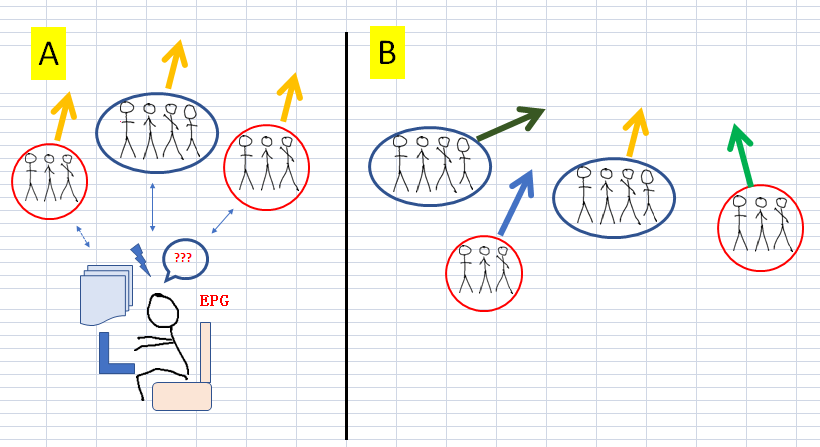
\includegraphics[width=10cm]{Diagram_20.png}

\begin{description}
\tightlist
\item[]
A：由公司的过程改进组（EPG）专员设计并执行过程改进的度量计划，包括收集哪些数据、如何收集以及如何分析。然后按计划收集各项目团队的数据，进行总体分析，并制定公司的改进方案。\\

B：将数据收集与分析的任务下放到各团队，让团队制定自己的改进方案。
\end{description}\strut
\end{minipage}}

项目经理：我认为度量与分析需要专业知识，要由专人来做，我选A。\\
我问：
但提供数据的人（图中EPG）需要很长时间才能收到反馈。例如，从团队成员提交里程碑数据，到项目经理填报，再由度量分析人员收集、整理多个项目的数据，可能需要一到两个月时间。再经过数据分析，管理层评审，最终到团队成员收到反馈可能共两三个月。由于每位提供数据者都希望尽快得到反馈，如果反馈的时间很长，那么团队成员还会有动力继续收集数据吗？\\
项目经理：估计确实可能会导致缺乏动力。\\
我：
无法确保数据的准确性，会导致分析没有意义。A场景很难确保数据的正确性。但B，因团队自己分析数据，会好些。\\
质量经理：从去年开始我们进行度量分析以来，就发现员工会对数据造假，导致结果失真。度量什么，他们就造假什么，所以我们想通过工具代替人工，不仅能提升效率，还能帮助判断数据是否合理。现在我们的主管很反感度量，因为每次度量就会有人造假------大家了解算法原理后，就开始造假。比如我们搞了红黑榜，但很多人聪明得很，就会想办法作弊。我们有很多数据统计分析，比如看测试用例与需求的比例。尽管客户发现的缺陷比例降低了，但由于我们对质量特别注重，产品经过多年的逐步演化，过程很复杂，导致软件缺陷的修复很耗时，客户不太满意。而且公司要求交付的频率要比以前高了很多，我们团队做这些分析都忙不过来，所以希望利用自动化工具加快速度。\\
我：确实有不少管理层误解了独立的用途，当度量数据被用于公司考核指标，便里面出现你说的情况。度量分析人员需要什么数据，提供数据的人都会按理想的指标填写，反正公司级的总体分析人员也无法验证数据的准确性。\\
除了数据收集问题，你们这种总体分析策略可能还有另一个问题：没有考虑各个项目的特性并不一样。现在你们对几十个项目的总体趋势进行分析，但每个项目的的差异可能很大，根本原因很可能不同。例如，你上次展示过一些测试数据，同样是测试用例比例数，你们采集的数据范围从最低的0.3到最高的超过200，但你们取平均值5.1来做分析。所以自动化工具不一定能帮到你。\\
但如果把数据分析下放到团队自己做，便灵活多了；也正因为他们有参与收集和分析讨论，过程改进组便可以节省很多沟通（数据收集）成本与失真。反而应该重新定位自己是内部老师，辅导团队怎么做好数据分析，效果会更好。\\
项目经理问：团队自己讨论便可以得到改进吗？不需要领导监督？\\
我：如果团队有能力，就应该放手让他们自己收集数据、利用数据进行分析并做出改进。但大部分团队还是没有做过度量分析，没有概念。所以质量经理应把自己重新定位为团队的教练，去辅导他们如何收集与分析数据，如下图的分工：右面的内部教练熟识各种度量分析技巧，辅导左面团队做改进。千万不要以为这项工作会比以前自己做分析更轻松，其实需要更熟悉整个过程，才能真正辅导好团队。要公司从定性管理提升到定量管理，最大的挑战是如何让项目团队动起来，所以应要让管理层了解并赞同需要让团队自主分析数据，自己寻找纠正措施。最终也要团队自己定目标，定计划，定期与上层汇报改进效果。例如，当你要健身锻炼减肥，也请了教练，最终因自己没有恒心，最终没有效果不应该把责任推卸到教练一样道理。\\
%\href{文件:Juran_f5.19.jpg}{600px}

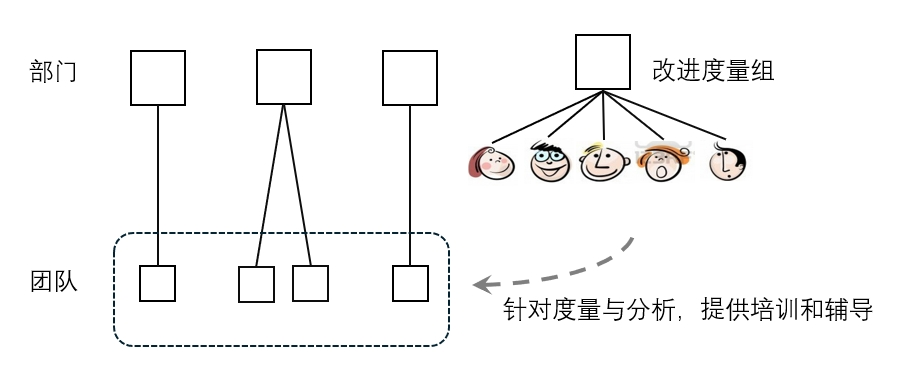
\includegraphics[width=10cm]{Juran_f519.jpg}

下一章会继续探索团队协作与分析根因；团队如何利用迭代冲刺数据，在敏捷冲刺回顾，做好根因分析，得到提升。

\hypertarget{ux9644ux4ef6}{%
\section{附件}\label{ux9644ux4ef6}}

\hypertarget{ux4e8cux516bux539fux52198020}{%
\subsection{二八原则(80/20)}\label{ux4e8cux516bux539fux52198020}}

帕里托(Pareto)
，16世纪意大利威尼斯人，他发现虽然威尼斯很富有，但财富并非平均分布，80\%财富在20\%手里，他也发现很多其他分布都非平均。

%\href{文件:ToolsParetoScreenshot_2023-06-02_191628.jpg}{400px}

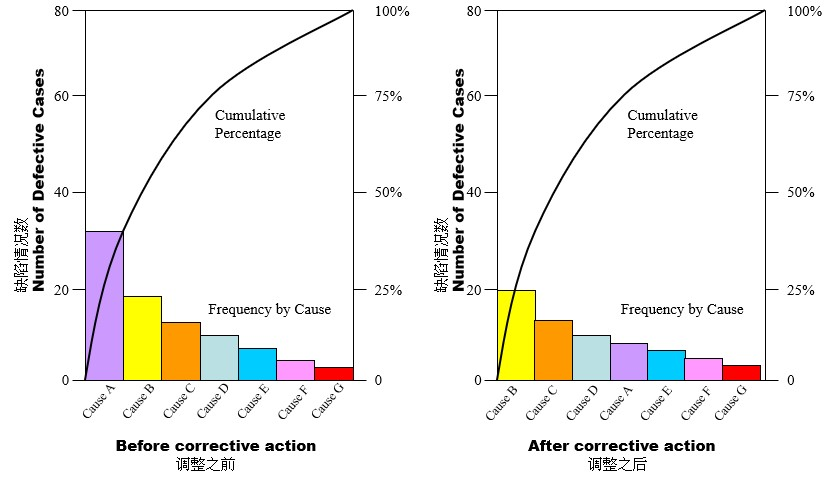
\includegraphics[width=10cm]{ToolsParetoScreenshot_2023-06-02_191628.jpg}

因为过程改进需要公司额外的资源投入，必须有针对性地找出最容易取得改进效果的原因，才可能拥有最大的成功机会。所以，应该利用二八原则去识别影响最大的几个因素.
以上图为例，原本A类问题出现最多，针对这类问题做过程改进之后，
A类问题就少了很多，下一轮便应针对最多的B类问题做改进。\\
有些人以为，只需要对某个维度做分析即可，并没有从多个维度进行分析。例如，某纸制产品工厂会计数据显示，8成的产品问题相关成本都归属于5类。\\
例如，某纸制产品工厂会计数据显示，因纸质量问题(Broke)被客户退货类的损失最大，共5560千美元，占总损失的61\%。（其他损失类包括材料成本高、生产线停顿等。）针对这类损失，发现里面八成是由6个产品引起（共有53个产品），共4480千美元，占5560的
80\%。针对这6个产品把损失按缺陷种类细分，发现B产品容易断裂缺陷(Tear)的占比最高，612千美元，我们就应该针对这一问题研究如何改善。

%\href{文件:162页替换图片.png}{600px}

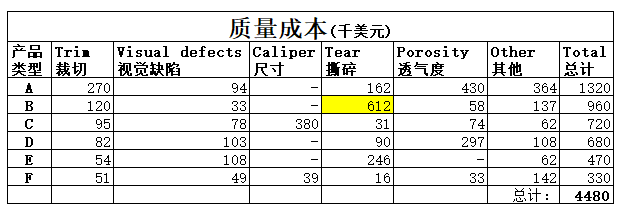
\includegraphics[width=10cm]{162页替换图片.png}

依据以上数据，可以按产品画帕累托图：

%\href{文件:微信截图_20241023163129.jpg}{600px}

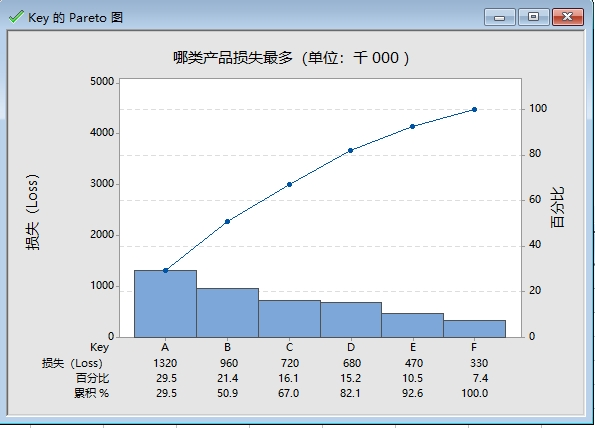
\includegraphics[width=10cm]{微信截图_20241023163129.jpg}

也可以按产品和缺陷类画帕累托图：

%\href{文件:微信截图_20241023163423.jpg}{600px}

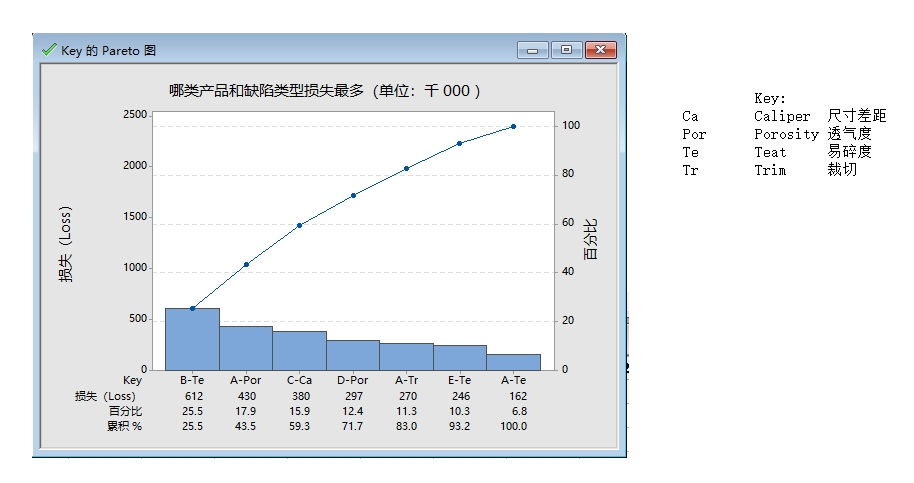
\includegraphics[width=10cm]{微信截图_20241023163423.jpg}

帕累托图除了能帮我们分析数据外，也能用于与高层沟通，让他们一目了然更好理解问题的主要源头，希望得到高层的支持。

\hypertarget{ux5f00ux53d1ux9879ux76eeux5de5ux4f5cux91cfux6210ux672cux5206ux5e03}{%
\subsection{开发项目工作量（成本）分布}\label{ux5f00ux53d1ux9879ux76eeux5de5ux4f5cux91cfux6210ux672cux5206ux5e03}}

参考Capers Jones先生2012的例子，汇总成以下比例：

%\url{文件:AR1成本占比.jpg}

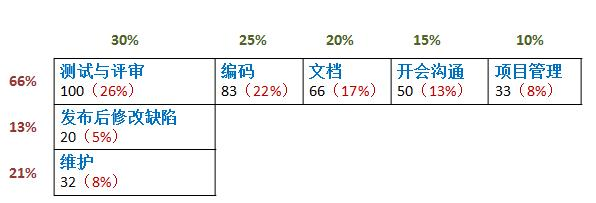
\includegraphics[width=10cm]{AR1成本占比.jpg}

测试与评审一般占开发工作量的30\%，测试与评审一般占总质量成本（包括发布后维护与改缺陷工作）的66\%，把所有工作量都加起来，测试与评审还是占最大(26\%)，编码第二
(22\%)。

\framebox{%
\begin{minipage}[t]{0.97\columnwidth}\raggedright
注意：测试与评审包括所有与缺陷相关的成本，包括单元测试、静态扫描、评审与相关的缺陷修正，而编码只包括设计与编写代码部分。例如有些人会觉得比例应该是开发30\%，测试和Bug修改25\%，需求和设计20\%，项目管理和沟通20\%，文档5\%。但如果按上面的定义，开发部分很可能已包括单元测试、静态扫描与改正缺陷工作，如把这些都归到测试评审里会变回类似上图的比例。
\strut
\end{minipage}}

\hypertarget{ux516cux53f8ux9ad8ux5c42ux4e0dux4e00ux5b9aux5173ux6ce8ux8d28ux91cf}{%
\subsection{公司高层不一定关注质量}\label{ux516cux53f8ux9ad8ux5c42ux4e0dux4e00ux5b9aux5173ux6ce8ux8d28ux91cf}}

\framebox{%
\begin{minipage}[t]{0.97\columnwidth}\raggedright
\textbf{问}：在传统 IT的
公司，无论是 缺陷(Bug)
率还是其他质量指标对业务的影响的相关性都不容易度量，只有重大事件才会让公司在客户面前失去信任，所以高层不会真正的重视质量。\\
\textbf{答}：理解，但软件BUG的暴露越往后，返工的工作量就越高，而且是几何级数的增加（例如在单元测试或评审发现都可以1人时内解决，在系统测试时发现通常要花20人时，在客户使用后才发现便更高）。但在很多IT公司，大部分缺陷都是在系统测试、甚至到验收测试才发现。如果能把软件缺陷的发现前移，把通过系统测试、验收测试发现的缺陷减半，便可以大量降低质量成本，提升开发生产率。所以我建议利用缺陷数估算返工的工作量来引起老板重视。（而不是仅仅说降低缺陷率）\\

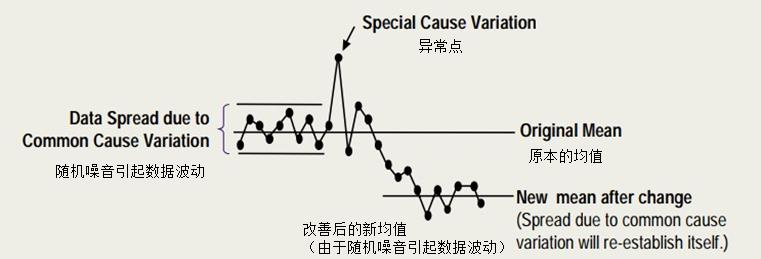
\includegraphics[width=10cm]{MGR_f11.jpg}
\strut
\end{minipage}}
